\chapter{Method}
\begin{figure}[h]
	\includegraphics[width=\textwidth]{Method.png}
	\caption{Steps of Change Point Analysis}
\end{figure}
\section{\label{section:Setting Simulation Environment}Setting Simulation Environment}
We setup the simulation environment to mimic the field experiments. So we distributed the resources as shown in figure $3.2$ . We had three different setups for three different species of ants. The number of agents were 12, 48 and 96. The total duration of each experiment was $90$ minutes (We collected data from field experiments for $90$ minutes only). The total arena size was $20\times20$ meter. We kept the arena into this size and bounded the agents to search in this arena.  The setup is varied for \textit{Maricopa} and \textit{Desertorum}. Table $3.1$ represents the environmental setup of simulations for \textit{P. rugosus}, \textit{P. maricopa} and \textit{P. desertorum}.
\begin{table}[h]
	\begin{tabular}{ |p{0.3\textwidth}|p{0.3\textwidth}|p{0.3\textwidth}| } 
		\hline
		\textbf{Species} & \textbf{Number of Seeds} & \textbf{Radius of Seed Distribution} \\
		\hline 
		\textit{P. rugosus} & 1024 & 5-10 meter\\ 
		\hline
		\textit{P. maricopa} & 128 & 1-3 meter\\ 
		\hline
		 \textit{P. desertorum} & 128 & 1-3 meter\\
		\hline
	\end{tabular}
	\caption{Environmental Setup of simulation for three species}
\end{table}
\begin{figure}[!h]
	\frame{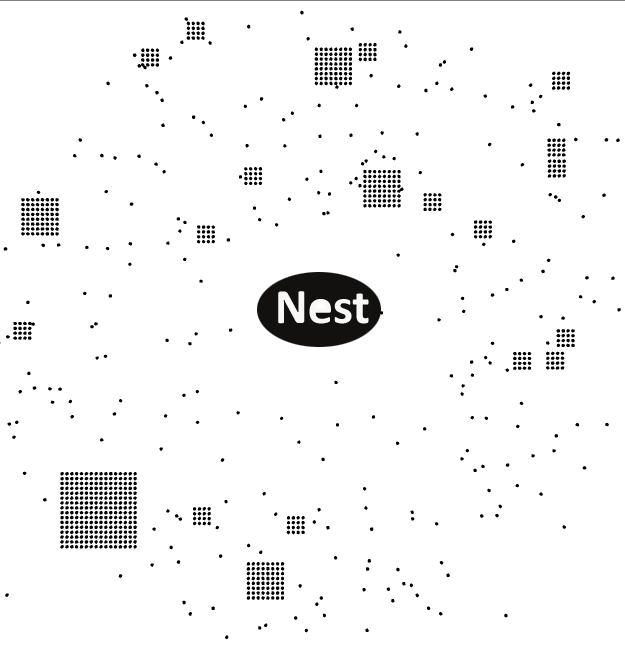
\includegraphics[scale=0.68]{ArGOS.jpg}}
	\caption{Example setup of a simulation environment for \textit{P. rugosus} with 1024 seeds three different types of piles. One large pile of $256$ seeds, four piles of $64$ seeds and sixteen piles of $16$ seeds. $256$ random seeds, are distributed uniformly inside the ring. }
\end{figure}
\section{\label{section:Tuning Parameters using Genetic Algorithm}Tuning Parameters using Genetic Algorithm}
   To analyze the data, we have tuned the parameters of CPFA. As stated above in the background study, enormous amount of parameters for CPFA can be used to evaluate the fitness. We have used the genetic algorithm to achieve the optimum set of parameters. We have divided the simulations into three categories to tune the GA for three different environments. 
   \begin{enumerate}
   	\item \textbf{Pheromone Only Parameters:}  For this type we have eliminated the use of site fidelity. Which means that the probability of using site fidelity is $20$, and remaining parameters are evolved using the GA. 
   	\item \textbf{Site fidelity Only Parameters:} In this type of experiment we eliminated the use of pheromone. For this case ants can only use site fidelity and random walk to collect resources
   	\item \textbf{Using Both site fidelity and pheromone:} This environment represents the actual field experiment condition in which agents use both site fidelity and pheromone along with the random walk.    	
   \end{enumerate}
For each type of environment, we have tuned the parameters to obtain maximum fitness using genetic algorithm where fitness is defined as maximizing the number of seeds collected in 90 minutes. Initially, we have created a population of one hundred colonies in the simulated environment. Each swarm\textquotesingle s foraging strategy is randomly initialized using the parameter setting mentioned in table $2.1$. The best genome is selected for crossover and mutation for next generation. We continued this process until we obtain the best fitness genome or parameter set. The GA is terminated either when the parameters are converged, or it reaches to generation $50$.\par  
For each swarm in a population, fitness is tested for four different random seeds. The value of random seed controls the variables of a simulation. After evaluation of each random seed for one parameter set, we have calculated the average seed collection to define the fitness of that particular swarm. These random seeds are basically numbers which are fixed for each generation. For each generation, we have selected four different numbers for the random seeds and then evaluated all the parameters for those values.\par  
To calculate the fitness for each parameter set it takes evaluating the fitness function for four times due to four different random seeds, which means for each generation it needs evaluating the objective function for $400$ times. So over $50$ generations, it will need $2000$ evaluations of the objective function. This can take a lot of time if we perform the evaluation sequentially.\par 
To remove this bottleneck, we have used multi-threading of genetic algorithm by evaluating multiple objective functions simultaneously. We have used GA Lib genetic algorithm package. The software for this work used the GAlib genetic algorithm package, written by Matthew Wall at the Massachusetts Institute of Technology. The MPI version was written by Andrew Rasmussen \url{https://github.com/andyras/GAlib-mpi/blob/master/LICENSE} who modified the code from \url{https://github.com/B0RJA/GAlib-mpi}.
The evolver.cpp file is used to initialize the GA parameters and pipe the parameters to the GA Lib.
Detail of initial parameter settings of genetic algorithm for three different setup is given in table $3.2$.
\begin{table}[h]
	\begin{tabular}{ |p{0.22\textwidth}|p{0.22\textwidth}|p{0.22\textwidth}|p{0.22\textwidth}| } 
		\hline
		\textbf{CPFA Parameters} & \textbf{Pheromone Only} & \textbf{Sitefidelity Only} & \textbf{All Parameters} \\
		\hline 
		Probability of Switching to Searching & U(0,1) & U(0,1) & U(0,1)\\ 
		\hline
		Probability of Returning to Nest & U(0,1) & U(0,1) & U(0,1)\\ 
		\hline
		Uniform Search Variation & (0, 4 PI) & (0, 4 PI) & (0, 4 PI)\\
		\hline
		Rate of Informed Searched Decay & E(20,0) & E(20,0) & E(20,0)\\
		\hline
		Rate of Site Fidelity & \textbf{E(20,20}) & E(20,0) & E(20,0)\\
		\hline
		Rate of Laying Pheromone & E(20,0) & \textbf{E(20,20}) & E(20,0)\\
		\hline
		Rate of Pheromone Decay & E(20,0) & \textbf{E(20,20}) & E(20,0)\\
		\hline
	\end{tabular}
	\caption{Initialization of seven parameters of CPFA for three different environments}
\end{table}
\section{\label{section:Generating Data Set for Analysis}Generating Data Set for Analysis}
 Once the parameters are tuned for three different environments, we have generated the data for our analysis using these parameter sets. For each of the experiment, we have extracted drop off time for each seed, location of each seed in the arena. Drop time is when it is dropped off at the nest. We have tagged each ant with distinct ID. For each seed, we also have extracted which ant has collected that seed. Also, we have tracked when the pheromone is laid, and followed, and when the site fidelity is followed. We have assigned distinct ID number to each pile so that when a pheromone trail is laid we can track which pile the trail is coming from.\par
 For each type of environment, we have simulated $500$ experiments and generated data mentioned above. We varied the value of random seed for each experiment while keeping the CPFA parameters constant for a particular environment. We also varied the position of seeds for each experiment. Each experiment was performed for $90$ minutes.\par 
 While generating the data for ``pheromone only parameters'', we did not extract any site fidelity data, because we tuned all the parameters not to use site fidelity data. Similarly, for ``site fidelity only'' experiments we did not extract any pheromone data as there was no pheromone. We have collected both site fidelity data and pheromone data when we have used both methods together for collecting resources.
 \section{\label{Analyzing The Foraging Data}Analyzing The Foraging Data}
 After generating all the data from the simulation, we have tried to observe how the ants collect seeds from different food distributions. We have observed that it takes some time for them to discover the larger piles. Once they discover it, they start to collect seeds from those piles. They use site fidelity and pheromone for this recruitment. Once they start collecting this seeds we see an increase in their foraging rate. So, we tried to detect those changes in their foraging rate by applying the change point detection algorithm. 
 \subsection{\label{Creating Timeline for each type of distribution}Creating Timeline for each type of distribution}
 We have studied each experiment separately to analyze the change in their foraging rate. For each experiment, we studied foraging rate for each type of pile individually. To study foraging rate for each pile we have created a time-line for each type of distribution. We have calculated foraging rate in overlapping windows, where each window has a fixed size and slided by a fixed time (such as 10 seconds) to create overlapping windows. Figure 3.3 shows the overlapping window for time-line. \par 
 \begin{figure}[h]
 	\includegraphics[width=\textwidth]{SlidingWindow.png}
 	\caption{An example of overlapping windows of foraging rate.}
 \end{figure}
 \begin{figure}[h]
 	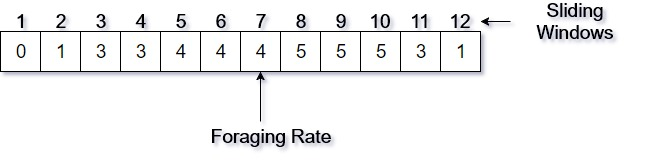
\includegraphics[width=\textwidth]{TimeLine.jpg}
 	\caption{An example of a timeline for a distribution where numbers at the top represent the sliding window number. Values in the boxes are the rate of collection of seeds per window.}
 \end{figure}
The length of the window is fixed to average time required for two round trips unless stated otherwise. For the simulated experiments it is 266 seconds. Sliding amount is fixed to 10 seconds. So if the experiment is for $90$ minutes ($5400$ seconds), we kept the length of the sliding windows for $266$ seconds and slided it by $10$ seconds, we get total $540$ sets of data where we calculated their foraging rate for a particular pile.\par 
 Once we have created the time-line for each experiment for a particular distribution of seeds we used change point detection algorithm to detect the change in the rate of collection of seeds. Another method we have created the timeline is by taking into consideration the change in the rate of foraging. In this method for creating the timeline instead of foraging rate, we take into consideration the change in foraging rate.\par
 \begin{figure}[h]
 	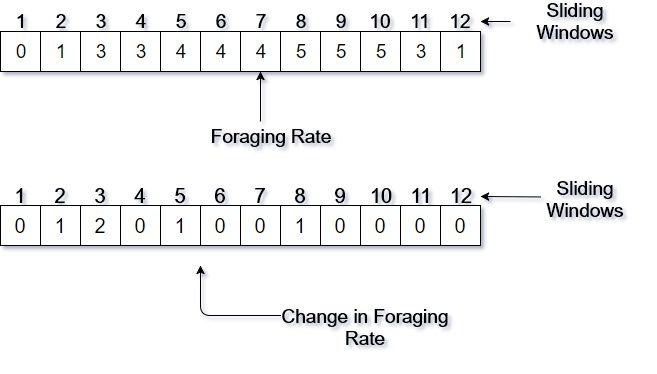
\includegraphics[width=\textwidth]{ChangeInForagingRate.jpg}
 	\caption{An example of timeline and change in foraging rate. The change in foraging rate is calculated by measuring the difference between the timeline windows}
 \end{figure}
\section{\label{section:Change Point Detection Algorithm}Change Point Detection Algorithm}
 The change point detection algorithm is divided into two parts. First part is the adding rate of collecting seeds to calculate the cumulative sum and detrend for smoothing. And the second part is applying the change point detection algorithm. We have used binary segmented cumulative sum method to determine the change points.
 \subsection{\label{Calculating the Cumulative Sum}Calculating the Cumulative Sum}
 The calculation of cumulative sum is basically adding the foraging rate in each window. Figure $3.6$ and algorithm $3.1$ demonstrates how the cumulative sum is calculated.\par
 \begin{figure}[h]
 	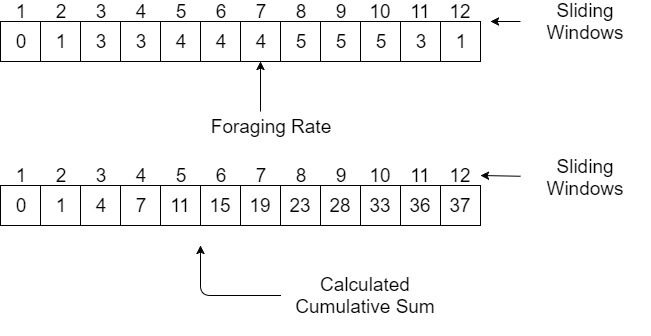
\includegraphics[width=\textwidth]{CumulativeSum.jpg}
 	\caption{This figure demonstrates how the cumulative sum is calculated from the timeline of foraging rate.}
 \end{figure}

 \begin{algorithm}[H]
 	\begin{algorithmic}[1]
 		\State Sum=0
 		\For{i=1:Number of Sliding Window} 
 			\State Sum= Sum + window(i)
 			\State CumulativeSum(i)=Sum
 		\EndFor
 		\caption{Pseudo code for calculating cumulative sum.}
 		\label{Pseudo code for calculating cumulative sum.}
 	\end{algorithmic}
 \end{algorithm}
 
 \subsection{\label{Detrending}Detrending}
 A time series trend is defined as a long-term change in the mean. The removal of a trend in a statistical or mathematical operation of time series is called detrending. It is often applied to remove features which are obsolete or unimportant. In time series analysis, detrending is also used in preprocessing step to prepare data set for further analysis.\par 
 There are several methods of detrending. Linear trends in mean can be truncated by subtracting a least-square-fit straight line. Different procedures are used for more complicated trend. For example, the cubic smoothing spline is commonly used in dendrochronology to fit and remove ring-width trend that might not be linear, or not even monotonically increasing or decreasing over time. It is important to understand the effect of detrending on spectral properties of time series before trying to remove the trend from the time series.\par 
 Before applying the change point detection algorithm, we have applied detrending algorithm to remove the trend from the time series. We used linear detrending and constant detrending to observe the effect of detrending in our time series data. Linear detrending removes the linear trend from the data where constant detrending removes the mean from the data. Figure $3.7$ demonstrates how linear and constant detrending affect the time series.\par
 \begin{figure}[H]
 	\begin{subfigure}{\textwidth}
 		\centering
 		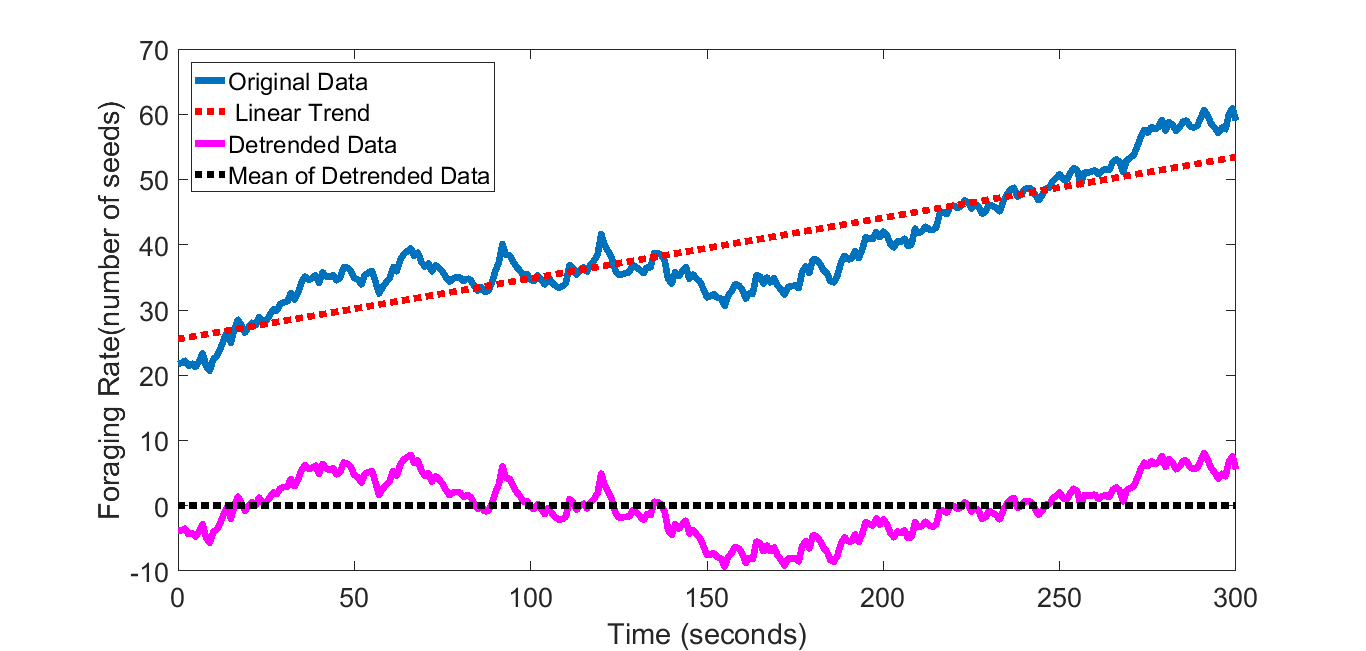
\includegraphics[width=\linewidth, height=0.3\textheight]{linearDetrending.jpg}
 		\caption{Linear Detrending}
 		\label{fig:Linear}
 	\end{subfigure}%
 	\\
 	\begin{subfigure}{\textwidth}
 		\centering
 		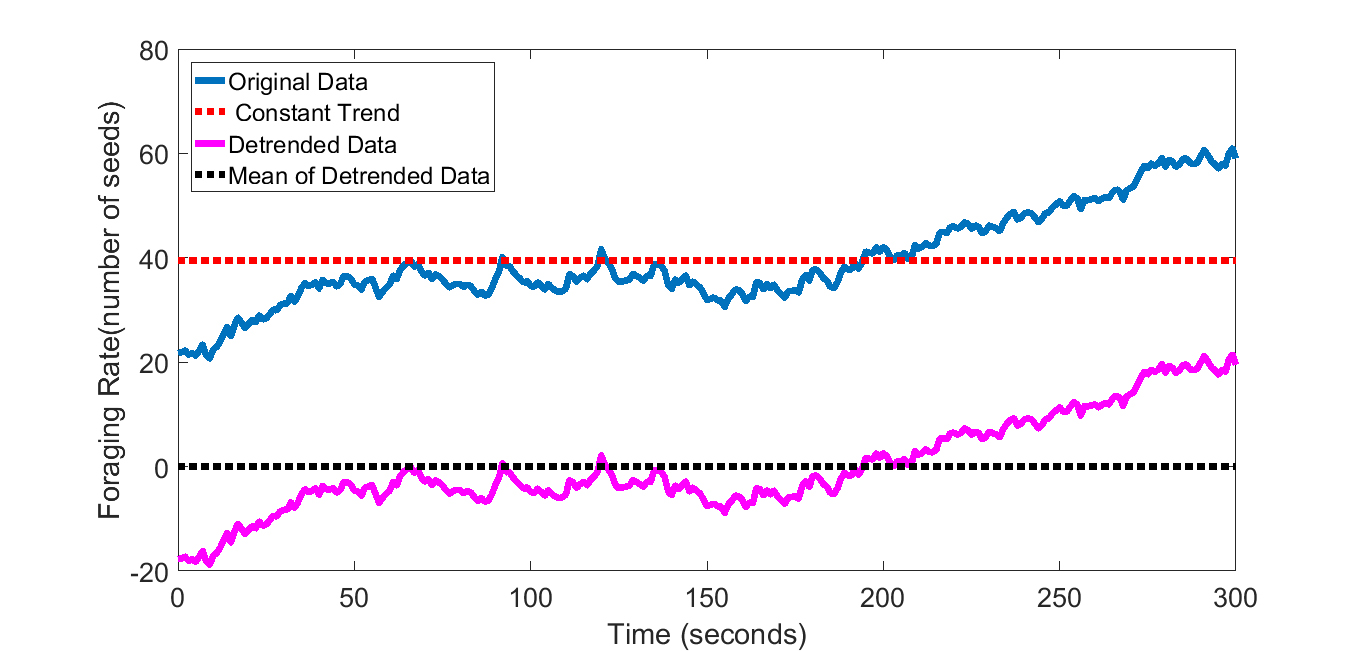
\includegraphics[width=\linewidth, height=0.3\textheight]{constantDetrending.jpg}
 		\caption{Constant Detrending}
 		\label{fig:Constant}
 	\end{subfigure}
 	\caption{An example of applying linear and constant detrending on the cumulative sum of a timeline from one simulated CPFA experiment.}
 	\label{fig:fig}
 \end{figure}
 \clearpage
\subsection{\label{Binary-Segmented Cumulative Sum}Binary-Segmented Cumulative Sum}
Binary Segmentation is one of the most established search method used for detecting the change point. This method extends any single change point method to multiple change points by iteratively repeating the method on different subsets of the sequence.\par 
To perform binary segmentation, we first apply the chosen single change point detection method to the entire data set, if no change point is found then we are done. If a change point is detected, call this $\tau$, then the data is split into two segments, timeline$[1:\tau]$ and timeline$[\tau+1:n]$. We then apply the single change point method to the two segments and repeat iteratively. We stop when no more change points are detected.\par
Binary segmentation is a very fast algorithm with complexity $O(n\log n)$ to detect the changes. But the major disadvantage of its computational speed is that it gives us only an approximation of changes. It is not guaranteed that the binary segmentation method will find us the optimum solution. Also due to iterative nature of this algorithm, it may not detect changes small changes. Thus, to verify the how well this method is performing, we have verified the results with the simulated data. 
The pseudo code for the binary segmentation algorithm is given in Algorithm $3.2$. 

\begin{algorithm}[!h]
	\begin{algorithmic}[1]
		 \State \algorithmicrequire A set of data of the form ($value_1$,$value_2$,$value_3$...)\\
		\qquad\quad\enspace A test statistic $\tau(.)$\\
		\qquad\quad\enspace An estimator of the changepoint position $\tau(.)$\\
		\qquad\quad\enspace A rejection threshold $\beta$
		\State\textbf{Initialize:} Let $C=\phi$, and $S=[1:n]$
		\While {$S\neq\phi$}
			\State Choose an element of S
			\State Denote this element as $[s,t]$
			\If{$ \tau (ys:t)<\beta $}
				\State remove$[s,t] from S$
			\EndIf
			\If {$\tau(ys:t)\geq\beta$}
				\State remove$[s,t] from S$
				\State calculate $ r=\tau(ys:t)+s-1 $, 
				\State add r to C
				\If {$r\neq s$}
					\State add $[s,r]$ to $S$
				\EndIf
				\If {$r=t-1$}
					\State $[r+1,t]$ to $S$
				\EndIf
			\EndIf
		\EndWhile	
		\caption{Pseudocode for Binary Segmented Mean Cumulative Sum}
		\label{Pseudocode for Binary Segmented Mean Cumulative Sum}
	\end{algorithmic}
\end{algorithm}
\clearpage
\section{\label{section:Verification of Change Points}Verification of Change Points}
As we have simulated data, and we know when the pheromones and site fidelities are used in simulations, we can certainly verify how efficient our change points detection algorithms are. So to check how efficient is our algorithms to detect change points, we divided the detection of change points into 4 categories.
\begin{itemize}
	\item \textbf{Catagory A or $\le 10$:} Change point detection within 10 seconds of pheromone laying events, 
	\item \textbf{Catagory B or $11-300$:} Change point detections within 11-300 seconds of pheromone laying events, 
	\item \textbf{Catagory C or $>300$:} Change point detections after more than 300 seconds of pheromone laying events and 
	\item \textbf{Catagory D or None:} Change point detected but no pheromone laying events has happened. 
\end{itemize} 
%So we have compared the results of four different methods based on this 4 categories using the data extracted from our simulation.
\clearpage
\section{\label{section:Applying the best method on Field Data}Applying the best method on Field Data}
We applied change point detection on 6 different types of the data set. This led us to evaluate the performance of change point detection algorithm for six different methods.
\begin{figure}[!ht]
	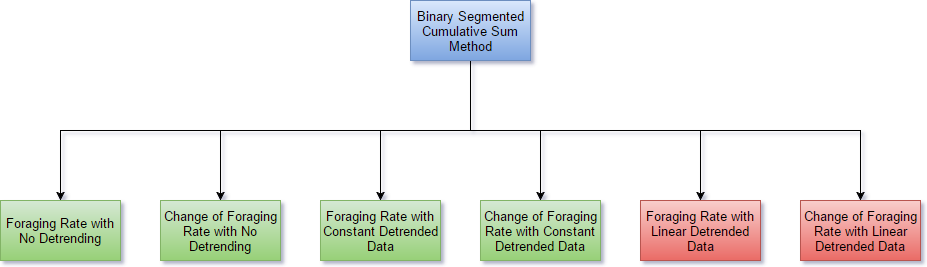
\includegraphics[width=\textwidth]{ChangePoint.png}
	\caption{Change point analysis on an alternate dataset}
\end{figure}
After validating six different methods that we have applied to simulation data. We select the best method for them based on the performance on six categories stated above, and we apply the best method in our field data.   

